\chapter{Algorithm design} \label{ch:alganalysis}
This chapter will explore the algorithm domain in the A$^3$ model. It is the domain marked on figure \vref{fig:a3alg}. This chapter will describe the two stereo vision algorithms, \textit{Efficient Edge Preserving Stereo Matching} (EEPSM) and \textit{Fast Cost-Volume Matching} (FCV). Lastly, a simulation of each algorithm is conducted and described and the results of these simulations are compared and from this, an algorithm is chosen.\\

\begin{figure}[ht!]
  \centering
  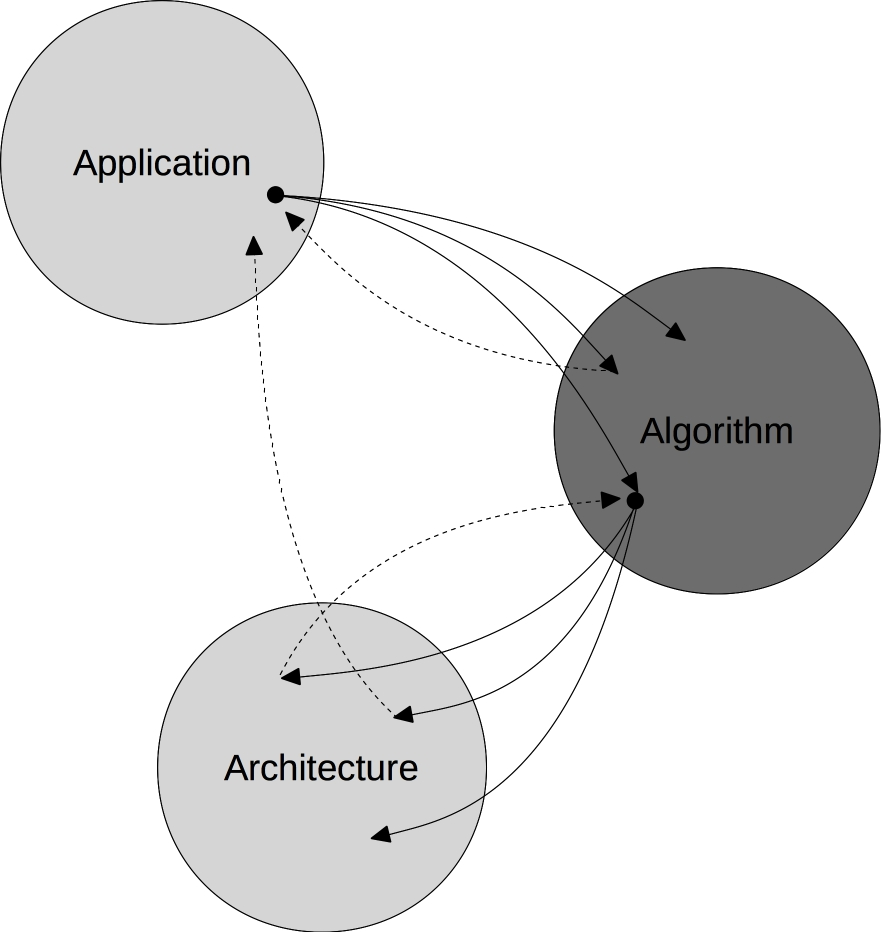
\includegraphics[scale=0.25]{figures/a3alg}
  \caption{A$^3$ model with the algorithm domain marked}
  \label{fig:a3alg}
\end{figure}

After the application analysis, a search for a fitting stereo vision algorithm can begin. During an internship at HSA systems a standard normalized cross-correlation (NCC) stereo matching algorithm was developed. An issue with the NCC algorithm is that it is not accurate near edges resulting in false matching around edges. For this project HSA systems wishes to find an algorithm which can be fast and is edge preserving. After some research, two algorithms were found. These algorithms are \textit{Efficient Edge Preserving Stereo Matching} and \textit{Fast Cost-Volume Matching}. The description of these algorithm comes from \cite{cciugla2011efficient} and \cite{hosni2013fast}. The pseudo code for the EEPSM is created by us while the FCV pseudo code comes from \cite{he2013guided} with some details added by us.

\section{Efficient Edge Preserving Stereo Matching (EEPSM):}\label{sec:eespm}
This algorithm is described in \cite{cciugla2011efficient}. This algorithm first calculates a cost for each pixel and disparity. This cost is a combination of the sum of absolute differences (SAD) and hamming distance of the census transform around each pixel. First the SAD is calculated:
\begin{flalign}
&& C^{SAD}_d(x,y) &=  \sum^3_{i=1}| I_l(x,y,i) - I_r(x+d,y,i) |  &&\label{eq:eepsmSAD}
\end{flalign}
where $i$ is the color (either red, green, or blue), $I_l(x,y,i)$ is a pixel in the left image or the reference image, and $I_r(x+d,y,i)$ is a pixel shifted by the disparity, $d$, in the right image or the target image.\\
This cost only uses the differences in color in a single pixel from each image and not a window around the pixel. Next the cost for a census transform is calculated.
\begin{flalign}
&& C^{CENSUS}_d(x,y) &= Ham(CT_l(x,y),CT_r(x+d,y)) && \label{eq:eepsmcomb}
\end{flalign}
Where $Ham(x_1,x_2)$ is the hamming distance between two bit strings and $CT(x,y)$ is the census transform around the pixel at $x,y$ of the grayscale version either the left image or the right image. The census transform converts the pixels in window around a center pixel into a bit string. Figure \vref{fig:census} shows a 3$\times$3 census transform. If the intensity (grayscale value) of a pixel is higher than the center then it is converted to 1 and 0 otherwise and then bits are inserted into a bit string. \\
\begin{figure}[ht!]
  \centering
  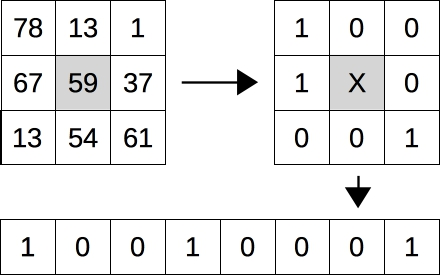
\includegraphics[height=3cm]{figures/census}
  \caption{Illustration of census transform}
  \label{fig:census}
\end{figure}

When the two cost values have been calculated they can be combined to a single cost value.
\begin{flalign}
&& C_d(x,y) &= \alpha \cdot C_d^{SAD} (x,y) + (1-\alpha)\cdot C^{CENSUS}_d (x,y) &&\label{eq:eepsmcost}
\end{flalign}
With the cost calculated the next step in the algorithm is to aggregate the cost. This is done in 3 steps. First step is to calculate permeability weights. Permeability is known from bio-medicine and describes the ability to transfer molecules through a cell membrane. The permeability weights are inspired by this and describes how well the color transfers from one pixel to another pixel and is expressed as:
\begin{flalign}
  && \mu(x,y) &= \min(e^{\dfrac{-\Delta R}{\sigma}},e^{\dfrac{-\Delta G}{\sigma}},e^{\dfrac{-\Delta B}{\sigma}}) &&\label{eq:premeability}
\end{flalign}
Where $\Delta R$, $\Delta G$, and $\Delta B$ is the difference in the specified color between two neighboring pixels and $\sigma$ is a smoothing factor. \\

The permeability weights should be calculated for each direction: up, down, left, and right and an example of the permeability of the downwards direction is shown in equation \vref{eq:permedown}.
\begin{equation}
\begin{split}
  \mu_{D}(x,y) = \min(&e^{\dfrac{-|I_l(x,y,1)-I_l(x,y-1,1)|}{\sigma}},\quad e^{\dfrac{-|I_l(x,y,2)-I_l(x,y-1,2)|}{\sigma}},\\
  &\hspace{2.9cm} e^{\dfrac{-|I_l(x,y,3)-I_l(x,y-1,3)|}{\sigma}}) \label{eq:permedown}
\end{split}
\end{equation}

The next step is to aggregate the cost in equation \vref{eq:eepsmcost} horizontally and this is achieved by using successive weighted summation (SWS) of the cost values along the left and right direction. The weights used in this summation will be the permeability weights for the right and left directions. The SWS for the right direction is expressed as:
\begin{flalign}
  && C^{R}_d (x,y) &= C_d(x,y)+ \mu_R (x-1,y) C^{R}_d (x-1,y) &&\label{eq:eepsmupdateR}\\
  && C^{R}_d (x,y) &= C_d(x,y)+ \sum_{i=1}^{x-1} \left(C_d(x-i,y)  \prod_{j=i}^{i} \mu_{R}(x-j,y) \right) &&\label{eq:eepsmupdateR2}
\end{flalign}
From equation \vref{eq:eepsmupdateR2} it is noticed that the cost, $C^R_d(x)$, will be affected by cost values from pixels to the left of point $x$ but the permeability weight ensures that only pixels close to point $x$ and with similar color will have a large influence. When there are large changes in color it is assumed that the pixels will belong to a new object and therefore it ensures that only pixels from the same object have an influence on the cost. \\

When aggregating the right SWS the algorithm starts in the left side and equation \vref{eq:eepsmupdateR} is used as an update rule while moving in the right direction. A similar update rule exists for the left SWS. When the left SWS and the right SWS have been performed then these can be combined to a horizontal SWS:
\begin{flalign}
  && C^{H}_d (x,y) &= C^{R}_d (x,y) + C^{L}_d (x,y)&&\label{eq:eepsmupdatehorz}
\end{flalign}
When the horizontal aggregation have been completed then vertical aggregation can be performed. The vertical aggregation is similar to horizontal aggregation but instead of using the cost $C_d(x)$ it uses the cost from horizontal aggregation, $C^H_d (x,y)$, and moves in the vertical directions, up and down. The two update rules for vertical aggregation and the combined vertical SWS is shown below:\\
\begin{flalign}
  && C^{U}_d (x,y) &= C^H_d(x,y)+ \mu_U (x,y-1) C^{U}_d (x,y-1) &&\label{eq:eepsmupdateU}\\
  && C^{D}_d (x,y) &= C^H_d(x,y)+ \mu_D (x,y+1) C^{D}_d (x,y+1) &&\label{eq:eepsmupdateD}\\
  && C^{V}_d (x,y) &= C^{U}_d (x,y) + C^{D}_d (x,y)&&\label{eq:eepsmupdatevert}
\end{flalign}

The cost from vertical aggregation, $C^V_d (x,y)$, will be influenced by the cost from pixels belonging to the same object as pixel at $(x,y)$ in greater or lesser degree. This cost can be used for minimization along disparity estimates with a winner take all approach. For occlusion perform a left-right cross check e.i. run the algorithm with the reference and target image changed around.\\

Through testing $\alpha$ in equation \vref{eq:eepsmcomb} is chosen to be \num{0.4}, the windows size of the census transform is chosen to be $3\times3$ and $\sigma$ in equation \vref{eq:premeability} is chosen to be \num{38.1}. These values have been determined through empirical observation.

\subsubsection*{EEPSM psuedo code} \label{sec:eepsmpsuedocode}
\textbf{Input:} \\
left image: $I_l$\\
right image: $I_r$\\
disparity estimate: $d$\\
\textbf{Output:} \\
filtering output: $q$\\
\textbf{Steps:}
\begin{enumerate}
  \item $C^{SAD}_d = f_{SAD}(I_l,I_{r,d})$\\
           $C^{CENSUS}_d = f_{Ham}(f_{CENSUS}(I_l),f_{CENSUS}(I_{r,d}))$
  \item $C_d = \alpha C^{SAD}_d + (1-\alpha) C^{CENSUS}_d$
  \item $\mu_D = f_{perme}(I_l,down)$ \\
           $\mu_U = f_{perme}(I_l,up)$ \\
           $\mu_L = f_{perme}(I_l,left)$ \\
           $\mu_R = f_{perme}(I_l,right)$
  \item $C^L = f_{SWS}(C_d,left)$\\
           $C^R = f_{SWS}(C_d,right)$
  \item $C^H = f_{SWS}(C^L,C^R,horizontal)$
  \item $C^U = f_{SWS}(C_d,up)$\\
           $C^D = f_{SWS}(C_d,down)$
  \item $C^V = f_{SWS}(C^U,C^D,vertical)$  
\end{enumerate}

\section{Fast Cost-Volume Matching (FCV):}
This algorithm is described in \cite{hosni2013fast}. As the algorithm in section \vref{sec:eespm} this algorithm calculates an initial cost and then aggregate this cost. The initial cost for this algorithm is also a combination of the sum of absolute differences and another cost. Instead of a cost based on census transform and hamming distance this algorithm uses difference in the gradient along the horizontal axis. The following equations show the different cost function for this algorithm and equation \vref{eq:fcvinitcost} shows the combined initial cost. First the SAD cost is calculated and this equation is similar to equation \vref{eq:eepsmSAD}.\\
\begin{flalign}
 && C^{SAD}_{d} (x,y) &= \sum^3_{i=1}| I_l(x,y,i) - I_r(x+d,y,i) |  && \label{eq:fcvSAD}
\end{flalign}
Then the gradient cost is calculated.
\begin{flalign}
  && C^{Grad}_{d} (x,y) &= \nabla_x I_l^{g} (x,y) - \nabla_x I_r^{g} (x+d,y) &&
\end{flalign}
Where $\nabla_x$ is the gradient along the x-axis and $I_l^g$ and $I_r^g$ is the grayscale version of each image. When these cost values have been calculated they can be combined to a single cost value:
\begin{flalign}
  && C_{d} (x,y) &= \alpha \cdot C^{SAD}_{d} (x,y) + (1 - \alpha) \cdot C^{Grad}_{d} (x,y) &&\label{eq:fcvinitcost}
\end{flalign}
When the initial cost has been found it will be aggregated. The fast cost-volume algorithm will aggregate the cost values using a guided image filter. 
\begin{equation}
  C'_d (x_i,y_i) = \sum_{x_j,y_j} W_{(x_i,y_i),(x_j,y_j)}(I) C_d (x_j,y_j)
\end{equation}
Where $C'_d (x_i,y_i)$ is the aggregated cost in pixel $x_i,y_i$ with disparity estimate, $d$, $x_j,y_j$ is pixels in a square window around $x_i,y_i$, and $W_{(x_i,y_i),(x_j,y_j)}(I)$ is the filter weights based on a guidance image, $I$. Section \vref{sec:guidedif} will describe how the filter weights are found.\\

This aggregate cost can then be used for minimization along the disparity estimates with a winner takes all approach. For finding occlusion a left-right cross check will also be used here.

\subsection{Guided Image Filter} \label{sec:guidedif}
This filter is described in \cite{he2010guided} and \cite{he2013guided} and this section simply summarizes their findings.\\
To describe the guided image filter a standard linear translation-variant filtering process is defined:
\begin{equation}
  q_i = \sum_j W_{i,j}(I)p_j
\end{equation}
Where $i$ and $j$ are pixel indexes, $q$ the filter output, $W_{i,j}(I)$ is a filter kernel which is function of a guidance image $I$, and $p$ is a input image.\\

The guided image filter is defined as a linear model between a guidance image, $I$, and a filtering output, $q$:
\begin{equation}
  q_i = a_k I_i + b_k, \forall i \in \omega_k \label{eq:gif1}\\
\end{equation}
where $i$ and $k$ is pixel indexes, $\omega_k$ is a square window centered at $k$, and $a_k$ and $b_k$ is linear coefficients which are assumed to be constant in the window, $\omega_k$. \\
How to determine $a_k$ and $b_k$ is described in \cite{he2013guided} and the solution is given by the following equations:
\begin{flalign}
  && a_k &= \dfrac{\frac{1}{|\omega|} \sum_{i \in \omega_k} I_i p_i - \mu_k \bar{p}_k}{\sigma^2_k + \epsilon} &&\label{eq:a_k}\\
  && b_k &= \bar{p}_k - a_k \mu_k && \label{eq:b_k}  
\end{flalign}
Where $|\omega|$ is the number of pixels in the window $\omega_k$, $\mu_k$ is the mean of $I$ in window $\omega_k$, $\bar{p}_k$ is the mean of input image $p$ in window $\omega_k$, $\sigma_k^2$ is the variance of $I$ in the window and $\epsilon$ is a regularization parameter which will penalize large $a_k$.\\

With $a_k$ and $b_k$ determined the filter output can be calculated:
\begin{equation}
  q_i = \frac{1}{|\omega|} \sum_{k|i \in \omega_k} (a_k I_i + b_k)
\end{equation}
$\sum_{k|i \in \omega_k} a_k = \sum_{k \in \omega_k} a_k$ because of symmetry in the square window and then the equation can be rewritten as
\begin{equation}
  q_i = \bar{a}_i I_i + \bar{b}_i
\end{equation}
Where $\bar{a}_i $ and $\bar{b}_i$ are the average coefficients for all windows that overlaps the pixel $i$ and are expressed as $\bar{a}_i = \frac{1}{|\omega|}\sum_{k \in \omega_k} a_k $ and $\bar{b}_i = \frac{1}{|\omega|}\sum_{k \in \omega_k} b_k$.\\

The guided image filter is used for its edge preserving property. The edge preserving property can be explained with the case where $I = p$ then:
\begin{flalign}
  && a_k &= \frac{\sigma_k^2}{\sigma_k^2 + \epsilon} &&\\
  && b_k &= (1-a_k)\mu_k &&
\end{flalign}
And if $\epsilon = 0$ then $a_k = 1$ and $b_k = 0$ but if $\epsilon > 0$ then two cases can occur. If the pixel is in an area where $I$ have a high variance in the window $\omega_k$ then $\sigma_k^2 \gg \epsilon$ and this results in $a_k \approx 1$ and $b_k \approx 0$. Instead if the pixel is in an area where $I$ is flat in the window $\omega_k$ then $\sigma_k^2 \ll \epsilon$ and this results in $a_k \approx 0$ and $b_k \approx 1$.\\
When these values are averaged then if the pixel are in a high variance area then the output is $q \approx p$ and if it instead is in a flat area the output is the average of surrounding pixels $q \approx p$.

\subsubsection*{FCV - grayscale - psuedo code}
\textbf{Input:} \\
left image: $I_l$\\
right image: $I_r$\\
disparity estimate: $d$\\
radius: $r$\\
epsilon: $\epsilon$\\
\textbf{Output:} \\
filtering output: $q$\\
\textbf{Steps:}
\begin{enumerate}
  \item $C^{SAD}_d = f_{SAD}(I_l,I_{r,d})$\\
           $C^{GRAD}_d = f_{GRAD}(I_l,I_{r,d})$
  \item $C_d = \alpha C^{SAD}_d + (1-\alpha) C^{GRAD}_d$
  \item $\mu_I = f_{mean}(I_l)$ \\
           $\mu_p = f_{mean}(C_d)$ \\
           $\rho_{II} = f_{mean}(I_l \cdot I_l)$ \\
           $\rho_{Ip} = f_{mean}(I_l \cdot C_d)$
  \item $\sigma_I = \rho_{II} - \mu_I \cdot \mu_I$\\
           $cov_{Ip} = \rho_{Ip} - \mu_I \cdot \mu_p$
  \item $a = cov_{Ip}/(\sigma_I + epsilon)$\\
           $b = \mu_p - a \cdot \mu_I $
  \item $\mu_a = f_{mean}(a)$\\
           $\mu_b = f_{mean}(b)$
  \item $q = \mu_a \cdot I_i + \mu_b$  
\end{enumerate}

The guided image filter described in this section and shown in the FCV psuedo code above is using grayscale images. To use color images then some changes have to be added to the guided image filter. Equation \vref{eq:gif1} will then become:
\begin{equation}
  q_i = \textbf{a}_k^T \textbf{I}_i + b_k, \forall i \in \omega_k \label{eq:gif1}\\
\end{equation}
Where $\textbf{I}_i$ is a 3$\times$1 color vector and $\textbf{a}_k$ is 3$\times$1 coefficient vector. Then the guided image filter will be:
\begin{flalign}
  && \textbf{a}_k = (\Sigma_k + \epsilon U)&^{-1} \left(\frac{1}{|\omega|} \sum_{i \in \omega_k} \textbf{I}_i p_i - \mu_k \bar{p}_k \right) &&\label{eq:a_k}\\
  && b_k &= \bar{p}_k - \textbf{a}_k^T \mu_k && \label{eq:b_k}  \\
  && q_i &= \bar{\textbf{a}}_k^T \textbf{I}_i + \bar{b}_i&&
\end{flalign}
where $\sigma_k$ is the 3$\times$3 covariance matrix of $\textbf{I}$ in window, $\omega_k$ and $U$ is the 3$\times$3 identity matrix.
\subsubsection*{FCV - color - psuedo code}
\textbf{Input:} \\
left image: $I_l$\\
right image: $I_r$\\
disparity estimate: $d$\\
radius: $r$\\
epsilon: $\epsilon$\\
\textbf{Output:} \\
filtering output: $q$\\
\textbf{Steps:}
\begin{enumerate}
  \item $C^{SAD}_d = f_{SAD}(I_l,I_{r,d})$\\
           $C^{GRAD}_d = f_{GRAD}(I_l,I_{r,d})$
  \item $C_d = \alpha C^{SAD}_d + (1-\alpha) C^{GRAD}_d$
  \item $\mu_{I,r} = f_{mean}(I_{l,r})$ \\
           $\mu_{I,g} = f_{mean}(I_{l,g})$ \\
           $\mu_{I,b} = f_{mean}(I_{l,b})$ \\
           $\mu_p = f_{mean}(C_d)$ \\
           $\mu_{Ip,r} = f_{mean}(I_{l,r}\cdot C_d)$ \\
           $\mu_{Ip,g} = f_{mean}(I_{l,g}\cdot C_d)$ \\
           $\mu_{Ip,b} = f_{mean}(I_{l,b}\cdot C_d)$
  \item $\sigma_{I,r,r} = f_{mean}(I_{l,r}\cdot I_{l,r}) - \mu_{I,r} \cdot \mu_{I,r}$\\
           $\sigma_{I,r,g} = f_{mean}(I_{l,r}\cdot I_{l,g}) - \mu_{I,r} \cdot \mu_{I,g}$\\
           $\sigma_{I,r,b} = f_{mean}(I_{l,r}\cdot I_{l,b}) - \mu_{I,r} \cdot \mu_{I,b}$\\
           $\sigma_{I,g,g} = f_{mean}(I_{l,g}\cdot I_{l,g})  - \mu_{I,g} \cdot \mu_{I,g}$\\
           $\sigma_{I,g,b} = f_{mean}(I_{l,g}\cdot I_{l,b}) - \mu_{I,g} \cdot \mu_{I,b}$\\
           $\sigma_{I,b,b} = f_{mean}(I_{l,b}\cdot I_{l,b}) - \mu_{I,b} \cdot \mu_{I,b}$\\
           $cov_{Ip,r} = \mu_{Ip,r} - \mu_{I,r} \cdot \mu_p$\\
           $cov_{Ip,g} = \mu_{Ip,g} - \mu_{I,g} \cdot \mu_p$\\
           $cov_{Ip,b} = \mu_{Ip,b} - \mu_{I,b} \cdot \mu_p$
  \item $\Sigma = f_{\Sigma}(\sigma_{I,r,r},\sigma_{I,r,g},\sigma_{I,r,b},\sigma_{I,g,g},\sigma_{I,g,b},\sigma_{I,b,b})$\\
           $cov_{Ip}= [cov_{Ip,r}, cov_{Ip,g}, cov_{Ip,b}]$\\
           $a = cov_{Ip}\cdot f_{inv}(\Sigma + epsilon\cdot U)$\\
           $b = \mu_p - a_r \cdot \mu_{I,r} - a_g \cdot \mu_{I,g} - a_b \cdot \mu_{I,b}$
  \item $\mu_{a,r} = f_{mean}(a_r)$\\
           $\mu_{a,g} = f_{mean}(a_g)$\\
           $\mu_{a,b} = f_{mean}(a_b)$\\
           $\mu_b = f_{mean}(b)$
  \item $q = \mu_{a,r} \cdot I_{i,r} +\mu_{a,g} \cdot I_{i,g}+\mu_{a,b} \cdot I_{i,b} + \mu_b$  
\end{enumerate}

Through testing $\alpha$ in equation \vref{eq:fcvinitcost} is chosen to be \num{0.11}, the windows size of the guided image filter is chosen to be $19\times19$ and $\epsilon$ in equation \vref{eq:a_k} is chosen to be \num{0.0001}. These values have been determined through empirical observation.

\section{Simulation and comparison}\label{sec:simucomp}
With each algorithm described the algorithms have been implemented in Python for simulation and comparison. The code for FCV is inspired by example matlab code from \cite{hosni2013fast}. The code for EEPSM is written by us using the description in this chapter. None of the Python implementations have been optimized further to ensure that run on multiple cores etc. It should also be noted that the simulations are using floating-point values.\\

The simulation were performed on a MacBook Pro, Retina, 15-inch (mid 2015). This machine have the following specifications.
\begin{itemize}
  \item OS: OS X El Capitan - version 10.11.6
  \item Processor: Intel\copyright  Core$^{\text{TM}}$ i7-4770HQ
  \item Memory: 16 GB 1600 MHz DDR3
  \item Python version: 2.7.12 | Anaconda 2.5.0
  \item Relevant Python packages: Numpy v1.10.4, matplotlib v.1.5.1
\end{itemize}

\begin{figure}[!ht]
  \centering
  \begin{subfigure}[t]{0.45\textwidth}
    \centering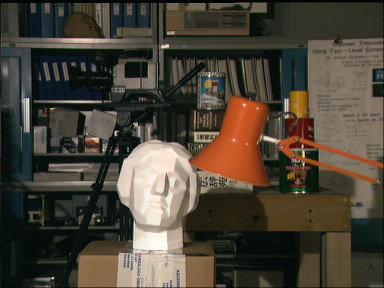
\includegraphics[height=5cm]{figures/tsul}
    \caption{Tsukuba \cite{Scharstein2002}\label{fig:tsu}}
  \end{subfigure}\hspace{0.5cm}
  \begin{subfigure}[t]{0.45\textwidth}
    \centering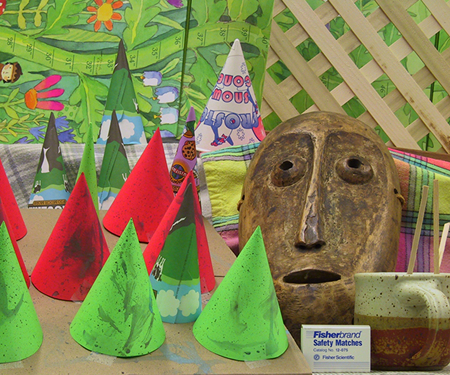
\includegraphics[height=5cm]{figures/conl}
    \caption{Cones \cite{Scharstein2003}\label{fig:cones}}
  \end{subfigure}
  \begin{subfigure}[t]{0.45\textwidth}
    \centering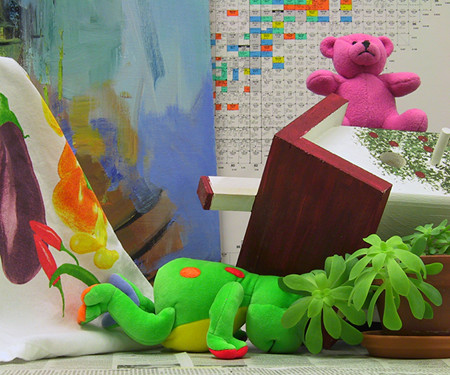
\includegraphics[height=5cm]{figures/tedl}
    \caption{Teddy \cite{Scharstein2003}\label{fig:ted}}
  \end{subfigure}\hspace{0.5cm}
  \begin{subfigure}[t]{0.45\textwidth}
    \centering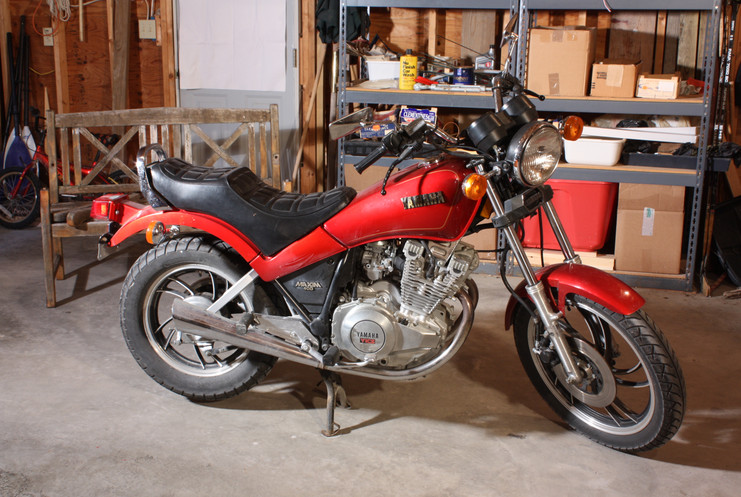
\includegraphics[height=5cm]{figures/motl}
    \caption{Motorcycle \cite{Scharstein2014}\label{fig:mot}}
  \end{subfigure}
  \caption{Middlebury data set - left images \cite{middlebury2016}\label{fig:middlebury}}
\end{figure}

For testing data sets from \cite{middlebury2016} are used. The stereo pairs are: Tsukuba, Cones, Teddy and Motorcycle and they are shown on figure \vref{fig:middlebury}. More information about the data sets is seen in appendix \vref{app:middlebury}.\\

The runtime and stereo matching quality results from the simulations are presented in table \vref{tab:runtime} and table \vref{tab:falseesti} while figures \vref{fig:tsuall} to \vref{fig:motall} shows resulting disparity maps. The results are discussed starting by discussing the visual result for each test set. Afterwards the calculated results, i.e run-time and number of false estimates, are discussed\\

\begin{figure}[ht]
  \centering
  \begin{subfigure}[t]{0.3\textwidth}
    \centering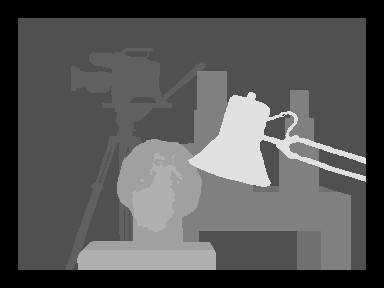
\includegraphics[width=5cm]{figures/tsu_gt}
    \caption{Ground truth \label{fig:tsu_gt}}
  \end{subfigure}\hspace{0.5cm}
  \begin{subfigure}[t]{0.3\textwidth}
    \centering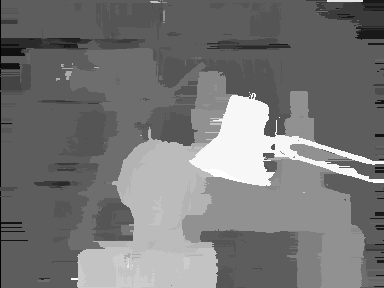
\includegraphics[width=5cm]{figures/tsu_fcv}
    \caption{FCV\label{fig:tsu_fcv}}
  \end{subfigure}\hspace{0.5cm}
  \begin{subfigure}[t]{0.3\textwidth}
    \centering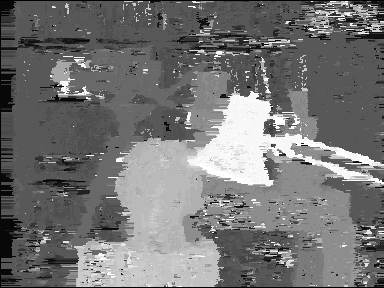
\includegraphics[width=5cm]{figures/tsu_eepsm1}
    \caption{EEPSM\label{fig:tsu_eepsm}}
  \end{subfigure}
  \caption{Tsukuba \cite{Scharstein2002}\label{fig:tsuall}}
\end{figure}

\begin{figure}[ht]
  \centering
  \begin{subfigure}[t]{0.3\textwidth}
    \centering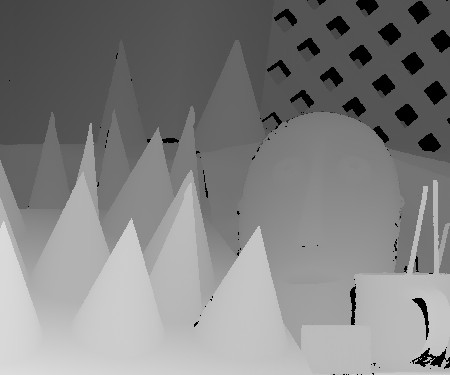
\includegraphics[width=5cm]{figures/con_gt}
    \caption{Ground truth \cite{Scharstein2003}\label{fig:con_gt}}
  \end{subfigure}\hspace{0.5cm}
  \begin{subfigure}[t]{0.3\textwidth}
    \centering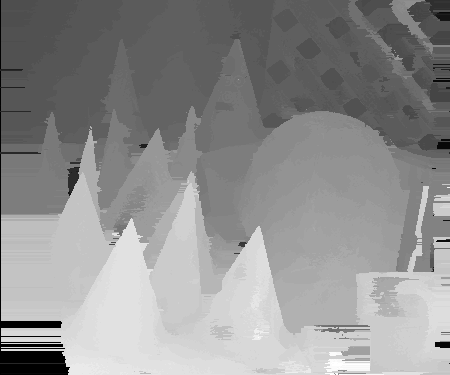
\includegraphics[width=5cm]{figures/con_fcv}
    \caption{FCV\label{fig:con_fcv}}
  \end{subfigure}\hspace{0.5cm}
  \begin{subfigure}[t]{0.3\textwidth}
    \centering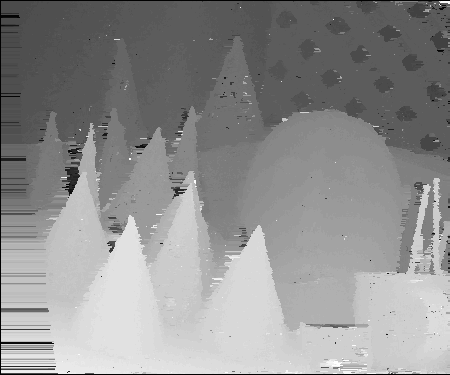
\includegraphics[width=5cm]{figures/con_eepsm1}
    \caption{EEPSM\label{fig:con_eepsm}}
  \end{subfigure}
  \caption{Cones \cite{Scharstein2003} \label{fig:conall}}
\end{figure}

\begin{figure}[ht]
  \centering
  \begin{subfigure}[t]{0.3\textwidth}
    \centering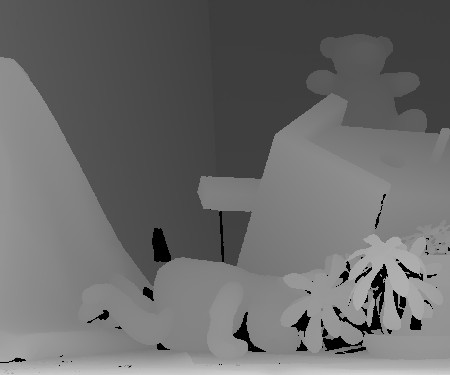
\includegraphics[width=5cm]{figures/ted_gt}
    \caption{Ground truth \cite{Scharstein2003}\label{fig:ted_gt}}
  \end{subfigure}\hspace{0.5cm}
  \begin{subfigure}[t]{0.3\textwidth}
    \centering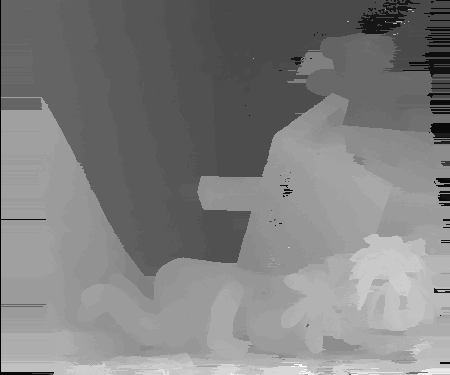
\includegraphics[width=5cm]{figures/ted_fcv}
    \caption{FCV\label{fig:ted_fcv}}
  \end{subfigure}\hspace{0.5cm}
  \begin{subfigure}[t]{0.3\textwidth}
    \centering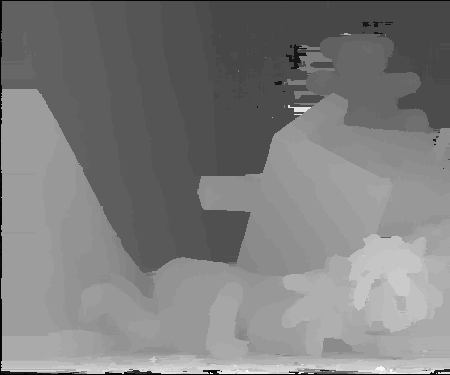
\includegraphics[width=5cm]{figures/ted_eepsm1}
    \caption{EEPSM\label{fig:ted_eepsm}}
  \end{subfigure}
  \caption{Teddy \cite{Scharstein2003} \label{fig:tedall}}
\end{figure}

\begin{figure}[ht]
  \centering
  \begin{subfigure}[t]{0.3\textwidth}
    \centering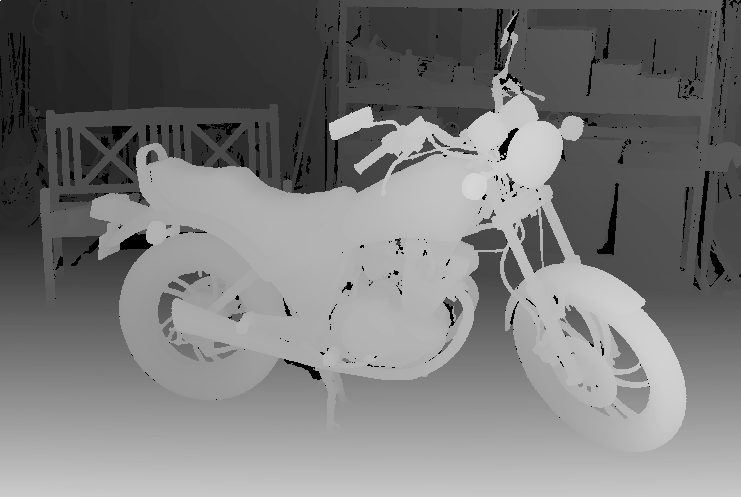
\includegraphics[width=5cm]{figures/mot_gt.png}
    \caption{Ground truth \cite{Scharstein2014}\label{fig:mot_gt}}
  \end{subfigure}\hspace{0.5cm}
  \begin{subfigure}[t]{0.3\textwidth}
    \centering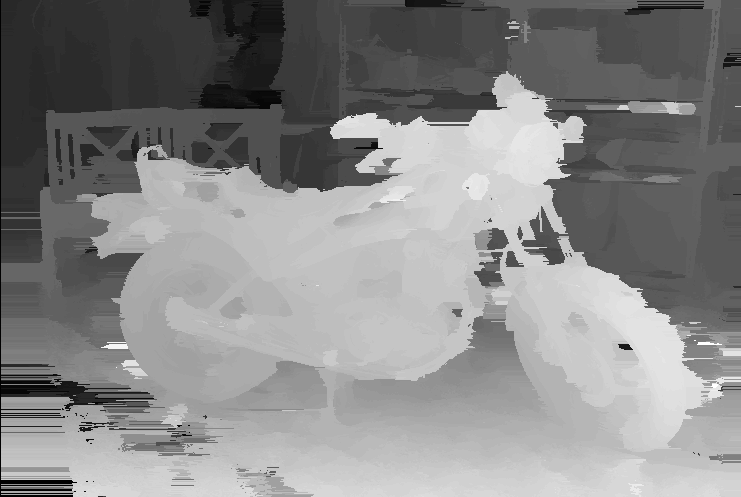
\includegraphics[width=5cm]{figures/mot_fcv}
    \caption{FCV\label{fig:mot_fcv}}
  \end{subfigure}\hspace{0.5cm}
  \begin{subfigure}[t]{0.3\textwidth}
    \centering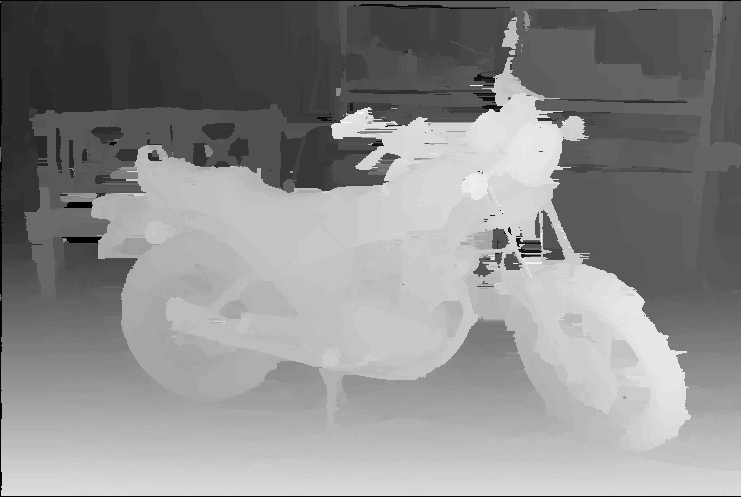
\includegraphics[width=5cm]{figures/mot_eepsm1}
    \caption{EEPSM\label{fig:mot_eepsm}}
  \end{subfigure}
  \caption{Motorcycle \cite{Scharstein2014}\label{fig:motall}}
\end{figure}

Looking at the Tsukuba test results on figure \vref{fig:tsuall} the FCV result seems better than the EEPSM result. The background seems more smooth on EEPSM result compared to the FCV result. Looking at the edges of objects FCV performs better in this test set. This is especially seen with the lamp. The silhouette of the lamp is sharper on the FCV result than on the EEPSM result and the sticks holding the lamp is missing in some areas in the EEPSM result.\\

Looking at the Cones test results on figure \vref{fig:conall} the EEPSM result seems better than the FCV result. The border occlusion filling in the left side are filled better on the EEPSM result. The occlusions are filled using the same method in both algorithms so any differences will come from the accepted matching results near the occluded area. Looking at the cones in the FCV result some of them have areas which jump in disparity value while the cones in the EEPSM result seems smooth. Some of the occlusions near the cones introduces more errors in the EEPSM result when compared to the FCV result. Looking at the box and cup in the lower right corner the result from EEPSM is better. The cup and box are smooth in EEPSM whereas in FCV there is some noise and in the EEPSM result, more of the sticks in the cup is found than in the FCV result. At last looking at the crisscross area in the right side of the background the EEPSM result is better. The holes in the surface are sharper in the FCV result but it have some errors when getting closer to the upper right corner whereas in the EEPSM result the whole surface is smooth.\\

Looking at the Teddy test results on figure \vref{fig:conall} the EEPSM result seems better than the FCV result. Again the border occlusion in the left side is filled better in the EEPSM result when compared to FCV. Both seems to have equal results when comparing the teddy in front and the chimney on the house. The roof in the FCV result have an area with false disparities and the edge of the roof near the gable is not as sharp as in the EEPSM result. The area behind/around the teddy on top of the house have errors in both results. The area is prone to giving errors due to the repetitive texture on the wall. The area to the left of the teddy is better in the FCV result while the area to the right is better in the EEPSM result.\\

Looking at the Motorcycle test results on figure \vref{fig:conall} the EEPSM result seems better than the FCV result. Once again the border occlusions have been filled better in the EEPSM algorithm. Looking at the ground, it is very smooth in the EEPSM result whereas in the FCV result large areas of the ground have errors like the lower left corner of the image. Looking at the background the FCV result has a large area with wrong disparity values while EEPSM seems smooth. The bench in the background is captured better in the FCV result where the holes and the silhouette are sharper when compared to the EEPSM result. Looking at the shelf unit in the background the FCV result has some areas with errors. Looking at the motorcycle is can be noticed that holes in the wheels and around the motor are present in either result. The side mirrors are captured better in the EEPSM result where they are sharper and one of the side mirrors isn't present in the FCV result. The rest of the motorcycle are more smooth in the EEPSM result while FCV have small areas with errors.\\

\begin{table}[ht!]
  \centering
  \begin{tabular}{l c c c }
    \toprule
    Image & Resolution & FCV & EESPM\\
    \midrule
    Tsukuba & $384\times288$ & \SI{180}{\second} & \SI{86}{\second}\\
    Teddy & $450\times375$  & \SI{542}{\second} & \SI{245}{\second}\\
    Cones & $450\times375$  & \SI{559}{\second}& \SI{260}{\second} \\
    Motorcycle &  $741\times497$  & \SI{1434}{\second}& \SI{625}{\second}\\
    \bottomrule
  \end{tabular}
  \caption{Run time for different stereo pairs \label{tab:runtime}}
\end{table}

\begin{table}[ht!]
  \centering
  \begin{tabular}{l c c c }
    \toprule
    Image & Resolution & FCV & EESPM \\
    \midrule
    Teddy & $450\times375$ & \SI{8.4}{\percent} & \SI{5.8}{\percent} \\
    Motorcycle & $741\times497$ & \SI{14.3}{\percent} & \SI{8.3}{\percent}\\
    \bottomrule
  \end{tabular}
  \caption{Percentage false disparity estimates \label{tab:falseesti}}
\end{table}

Table \vref{tab:runtime} shows the runtime for each algorithm process each test set. From this, it is seen that EEPSM is more computationally efficient when compared with FCV. EEPSM is more than twice as fast as FCV at processing each test set. The main difference in runtime comes from the aggregation of the initial cost values. The SWS in EEPSM is less complex than the guided image filter in FCV.\\

Table \vref{tab:falseesti} shows the number falsely estimated pixels. As seen the EEPSM algorithm performs better in this area too. One of the main contributors to the difference in percentage of errors seems to be the errors near borders and the ground in the motorcycle test set.

\section{Theoretical Complexity} \label{sec:theorycomplex}
The simulations of the algorithms might have unknown factors which can affect the performance e.g. the programmers knowledge of the algorithms and programming skills. To ensure a more precise estimation of the performance of the algorithms the theoretical computational complexity have been calculated. \\

Table \vref{tb:theocompl} shows the number of addition, multiplications, divisions and comparisons used per pixel. \\
It should be noted that the exponential function in the EEPSM algorithm is not a simple function to implement in hardware therefore it will be approximated here with a power series:
\begin{equation}
  e^x = \sum_{n=0}^{\infty} \dfrac{x^n}{n!} = 1 + x + \dfrac{x^2}{2!} + \dfrac{x^3}{3!} + \dots \label{eq:exppowser}
\end{equation}
In section \vref{sec:expfunc} the challenges of implementing exponential function in hardware is discussed and from this section it is found that 23 terms of the power series is needed to achieve an approximation error $\leq 0.001$ for values in the interval $[ -\dfrac{255}{38.1}; \dfrac{0}{38.1}]$. The power series approximation with 23 terms is used in the calculation of the theoretical complexity instead of the exponential function.
\begin{table}[ht!]
  \centering
  \begin{tabular}{c c c c c c}
    \toprule
    & type & add/subtract & multiplication & division \\
    \midrule
    EEPSM & C & $8768 \cdot N$ & $5460 \cdot N$ & $0$ \\
    & G & $7372 \cdot N$ & $3133 \cdot N$ & $0$ \\
    FCV & C & $296031 \cdot N$ & $63630 \cdot N$ & $303 \cdot N$ \\
    & G & $104838 \cdot N$ & $16059 \cdot N$ & $303 \cdot N$ \\
    \bottomrule
  \end{tabular}
  \caption{Complexity of each algorithm, where N is the number of pixels}
  \label{tb:theocompl}
\end{table}
From the table it is noticed that the FCV requires a lot more operations per pixel when compared to EEPSM. This is mainly due to the guided image filter which have a window size of $19\times 19$ which results in a lot of addition and multiplication for each single result. It is also seen that with EEPSM the change between color and grayscale doesn't reduce the number of operations by a large factor while with FCV this change reduces the number of operations by a lot. This is due to the EEPSM algorithm only using color during initial cost and finding permeability weights while in FCV the use of color makes the guided image filter require far more operations. \\

I/O communication can also have a influence on the performance hence the memory reads and writes for each algorithm have also been calculated and the result is shown in table \vref{tb:memuse}. It should be noted that when calculating reads and writes for the FCV that the mean function is assumed to be a running window.\\
\begin{table}[ht!]
  \centering
  \begin{tabular}{c c c c c }
    \toprule
    & type & reads & writes \\
    \midrule
    EEPSM & C & $6402 \cdot N$ & $2731 \cdot N$  \\
    & G & $5778 \cdot N$ & $2731 \cdot N$ \\
    FCV & C & $9740 \cdot N$ & $5766 \cdot N$ \\
    & G & $4861 \cdot N$ & $3033 \cdot N$ \\
    \bottomrule
  \end{tabular}
  \caption{Memory reads and writes used by each of the algorithms, where N is the number of pixels}
  \label{tb:memuse}
\end{table}

From table \vref{tb:memuse} it is seen that the change from color to grayscale in EEPSM doesn't change the number of reads by much and the number of writes remains the same. This is due to the EEPSM algorithm only using color in a few functions. On the other hand, it is noticed that the FCV algorithm reduces the number of reads and writes by much. This is because of color being used in a lot of functions in the guided image filter. When using color EEPSM uses less I/O communication when compared to FCV while when using grayscale FCV uses fewer reads than the EEPSM algorithm but still uses more writes. From the results in this table EEPSM generally performs better.

\section{Choosing an algorithm}
One of the algorithms described in this chapter should be chosen for further implementation on a FPGA. This choice is based on the results from section \vref{sec:simucomp} and section \vref{sec:theorycomplex}. \\

Starting with the computational efficiency table \ref{tab:runtime} shows that the Python implementation of the EEPSM algorithm is more than twice as fast as the FCV algorithm (run-time is reduced by 52-56\%). To ensure that these results are not affected by unknown factor e.g. the programmer's programming skills, the theoretical computational complexity is also used. Table \vref{tb:theocompl} and \vref{tb:memuse} shows the number of operations and I/O communication per pixel. This shows the same result. The reason that EEPSM is faster is due to the aggregation each uses. The SWS requires far fewer operations when compared to the guided image filter especially when using color.\\

The quality of the resulting disparity map should also be taken into consideration when choosing an algorithm. The visual inspection of the results shows that EEPSM algorithm generally results in better disparity maps in all except for one of the test sets which is the Tsubuka test set. But this test set is the least important since it is the set with the lowest resolution and the images for a prototype will have a much higher resolution. In some situations, FCV gives a bit better result than the EEPSM algorithm i.e. the holes in the bench in figure \vref{fig:motall}. Table \vref{tab:falseesti} shows that the EEPSM algorithm results in disparity maps which are closer to the ground truth when compared to the FCV algorithm results (between 31-42\% fewer false estimates).\\

Referring to the cost function from chapter \ref{ch:req} the two main factors to consider when choosing an algorithm is time and stereo matching quality with time having the highest priority. Considering these two factors and the results which are summarized in this section the EEPSM algorithm is chosen.

\section{Wrap-up}
Two edge preserving stereo vision algorithms have been described. The algorithms have been simulated using Python and floating point. To support the results from the simulations their theoretical complexities has been calculated. The results show that the EEPSM algorithm has a lower execution time and matches better than the FCV algorithm. Considering these results and the cost function in chapter \ref{ch:req} the EEPSM algorithm is chosen to be implemented on a FPGA. 